%%%%%%%%%%%%
%
% $Autor: Wings $
% $Datum: 2019-03-05 08:03:15Z $
% $Pfad: SetUp.tex $
% $Version: 4250 $
% !TeX spellcheck = en_GB/de_DE
% !TeX encoding = utf8
% !TeX root = manual 
% !TeX TXS-program:bibliography = txs:///biber
%
%%%%%%%%%%%%

\chapter{System Setup and Configuration}

This chapter provides detailed steps to set up the hardware and software required for the Face Recognition Access Control System. Follow the instructions carefully to ensure a smooth installation, configuration and debugging process.

\section{Software Requirements}
\begin{itemize}
	\item \textbf{Python 3.10 or latest version:} Required for running scripts and managing data preprocessing or additional configurations.
	\item \textbf{Arduino CLI:} Essential for managing Arduino board configurations, libraries, and code deployment via the command line.
	\item \textbf{Edge Impulse CLI:} Required for running the model in debug mode and streaming real-time results.
\end{itemize}

\section{Installation Steps}

\begin{enumerate}
	\item \textbf{Python Installation:}
	\begin{itemize}
		\item Download the latest version of Python (3.10 or above) from \href{https://www.python.org}{https://www.python.org}.
		\item Run the execution file and follow the installation instructions for your operating system.
		\item During installation, check the box to add Python to your system's PATH.
	\end{itemize}
	
	\item \textbf{Arduino CLI Installation:}
	\begin{itemize}
		\item Visit \href{https://arduino.github.io/arduino-cli}{https://arduino.github.io/arduino-cli} to download the Arduino CLI for your operating system.
		\item Extract the downloaded files to a preferred location.
		\item Add the CLI path to your system's PATH variable.
		\item Verify installation by running \SHELL{arduino-cli version} in your terminal or command prompt.
	\end{itemize}
	
	\item \textbf{Edge Impulse CLI Installation:}
	\begin{itemize}
		\item Install Node.js from \href{https://nodejs.org}{https://nodejs.org}.
		\item Open a terminal and run: \SHELL{npm install -g edge-impulse-cli}.
		\item Verify installation by running: \SHELL{edge-impulse-daemon --version}.
	\end{itemize}
	
	\item \textbf{Clone the Project Repository:}
	\begin{itemize}
		\item Clone the software repository containing the project code by running:  
		\texttt{git clone https://github.com/project-repository.git}
		\item Review the provided files and ensure all dependencies are properly configured.
	\end{itemize}
\end{enumerate}

\section{Initial Configuration}

\begin{enumerate}
	\item \textbf{Python Configuration:}
	\begin{itemize}
		\item Install the required Python packages by running: \texttt{pip install -r requirements.txt}.
		\item Ensure all packages are installed successfully.
	\end{itemize}
	
	\item \textbf{Arduino CLI Configuration:}
	\begin{itemize}
		\item Add the Arduino board manager URL by running:  
		\\ \SHELL{arduino-cli config add board\_manager.additional\_urls}
		\SHELL{https://downloads.arduino.cc/packages/package\_index.json}.
		\item Update the board index: \\ \SHELL{arduino-cli core update-index}.
		\item Install the Portenta H7 board core:
		\\ \SHELL{arduino-cli core install arduino:mbed\_portenta}.
	\end{itemize}
	
	\item \textbf{Edge Impulse Configuration:}
	\begin{itemize}
		\item If you want to retrain or customize the model via Edge Impulse Studio:
		\item Connect the Portenta H7 to your computer via USB.
		\item Run the following command to start the daemon:  
		\SHELL{edge-impulse-daemon}.
		\item Log in to Edge Impulse Studio when prompted and link your device.
		\item Use Edge Impulse Studio to update or retrain the model with your input dataset, then export it as a file \FILE{.zip} for deployment in Arduino CLI.
	\end{itemize}
\end{enumerate}


\chapter{Getting Started}

\section{Connecting the Hardware}
\begin{enumerate}
	\item Mount the Vision Shield to the Portenta H7 carefully.
	\item Insert the Micro SD card into the Vision Shield.
	\item Connect the Portenta H7 to a USB-C power adapter (5V, 2A).
	\item Check the LED indicator on the Portenta H7, that indicates the device is powered ON.
\end{enumerate}

\section{Execute the Model}

\begin{enumerate}
	\item Once the Portenta H7 is powered ON, the pre-installed model will automatically initialize and be ready to run.
	\item Open a terminal on your computer and enter the following command to start the inference process: \\ \SHELL{edge-impulse-run-impulse}
	\\This will run the model on the Portenta H7 and provide real-time recognition results in the terminal as shown in figure ~\ref{inference}.
	\item If you need detailed logs or debugging information, use the debug mode by running the following command:
	\\ \SHELL{edge-impulse-run-impulse --debug}
	\\This mode will display additional information, such as inference timing, data acquisition details for visualization as shown in the figure ~\ref{debug}.
\end{enumerate}

\begin{figure}
	\begin{center}
		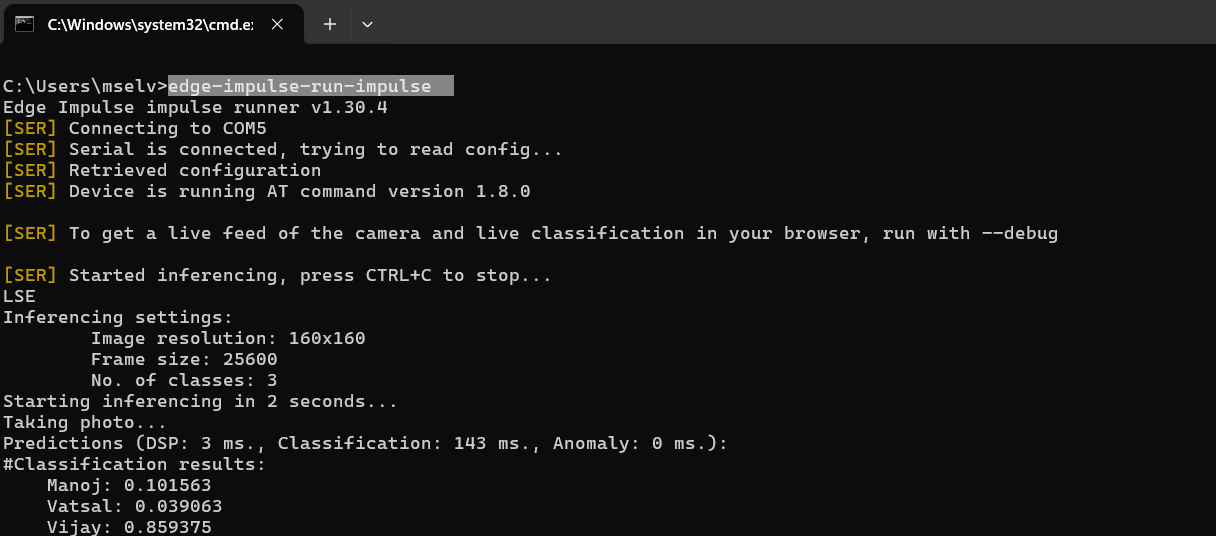
\includegraphics[width=0.7\linewidth]{Images/run_impulse.png}
		\caption{Running the inference}
		\label{inference}
	\end{center}
\end{figure}

\begin{figure}
	\begin{center}
		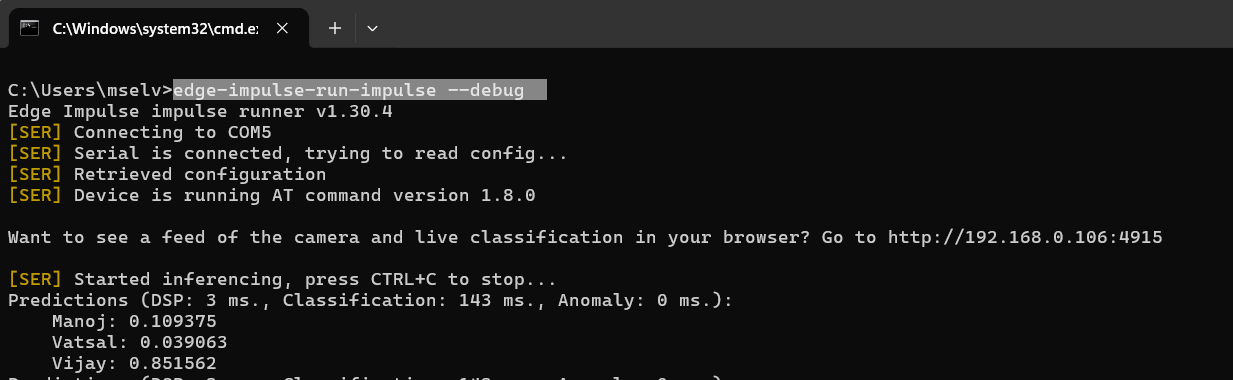
\includegraphics[width=0.7\linewidth]{Images/impulse_debug.png}
		\caption{Debug Mode}
		\label{debug}
	\end{center}
\end{figure}